\documentclass[9pt,twoside,lineno]{pnas-new}
% Use the lineno option to display guide line numbers if required.

\templatetype{pnassupportinginfo}

\title{The structure of developmental variation in early childhood}
\author{Ben Stenhaug, Nilam Ram, and Michael C. Frank}
\correspondingauthor{Ben Stenhaug\\E-mail: benastenhaug@gmail.com}

\begin{document}

%% Comment out or remove this line before generating final copy for submission; this will also remove the warning re: "Consecutive odd pages found".
%% \instructionspage

\maketitle

%% Adds the main heading for the SI text. Comment out this line if you do not have any supporting information text.
\SItext

\section*{S1. Additional information for Study 1 and Study 2}

One benefit of the item response theory is that item parameters can be examined to better understand their behavior. As an example, Figure \ref{fig:curves} shows the item response curves for nine of the 414 milestones based for the 1F fit to the survey data. The variety of curves show that some milestones load more or less heavily onto the estimated factors—for example, the probability of "points to familar objects" increases sharply when a child's factor score nears zero whereas "babbles if simulatiog conversation" shows no relationship to the estimated factor. The curves also show that the difficulty, or at what factor score a child is likely to reach a milestone, varies greatly by milestone as well—for example, chldren are able to "go from standing to sitting" at relatively low factor scores whereas having a significant probability of "playing board games" requires a much higher factor score.
\\\\
Ceiling effects are a potential threat to the validity of our method for examining age-related differences in within-person coupling of factor scores. In particular, if the factors were to reach a ceiling, then associations between residuals from the developmental trends would not have a meaningful interpretation. Figure \ref{fig:rawp} shows that ceiling effects are not a concern as the raw percent of milestones responded to that the child has reached stays relatively constant over the age-span as a result of milestones becoming more advanced for older children.
\\\\
In study 2, we estimated coupling as a function of age under a 2F measurement model which made the factors easier to interpret and the method more straightforward. However, study 1 found that the Kinedu data is best described by more than two dimensions. Figure \ref{fig:three} shows the results of the same process using a 3F measurement model. As evidence for the differentiation hypothesis we find negative coupling over the age span between factors 1 and 2 as well as factors 1 and 3.

\section*{S2. Analysis of data from the Survey of Well-being of Young Children (SWYC)}

In our pre-registration (https://osf.io/5426p/) we described our plan to use an additional dataset that we did not report on in the paper. The dataset comes from adminstrations of the Survey of Well-being of Young Children (SWYC). The SWYC data has a number of properties that we now realize make it a poor candidate for the paper's research questions.
\\\\
\textit{Many versions:} A different version of the SWYC is administered depending on the child's age, and the types of milestones from version to version sometimes vary greatly. Table \ref{tab:swyc} contains a row for each version and the last four columns show the number of milestones by category for each version. By comparison, each parent in the Kinedu survey data responded to all milestone questions regardless of their child's age.
\\\\
\textit{Low sample sizes:} Each SWYC version contains exactly 10 milestones and we have data from only 74-329 children for each version. Table \ref{tab:swyc} shows these sample sizes. By comparison, the Kinedu survey data contains data for ~2k children to all 414 milestone questions.
\\\\
\textit{Cross-sectional:} For the vast majority of children in the SWYC data, we have data from a single occasion. This makes longitudinal examination of the differentiation hypothesis impossible. By comparison, we were able to use the Kinedu app data to see how many childrens' development changed over time.
\\\\
We came to these realizations as we analyzed the SWYC data. For transparency, we describe the SWYC data, methods (which mirrors Study 1), and results here.

\subsection*{Data}
Data comes from 2,186 administrations of the Survey of Wellbeing of Young Children (SWYC). This data differs from the data from Kinedu, Inc in a number of important ways. First, the SWYC is a well-known and trusted instrument developed by the National Institute for Children’s Health Quality. Second, the SWYC data was reported by clinicians whereas the Kinedu, Inc. data was reported by parents/guardians. Third, the SWYC questionnaire has a number of different versions depending on the age of the child. In comparison, The Kinedu, Inc. data came from a survey where each parent responded to all 414 milestone questions regardless of the child’s age. Fourth, the SWYC uses a likert scale for each question whereas the Kinedu, Inc. data contains only binary responses. We took the following pre-processing steps.
\\\\
\textit{Multiple administrations for a single child:} The SWYC data contains 2,062 children. 113 of these children have multiple SWYC administrations in the dataset. So that each child represents a single datapoint, we considered only the first SWYC administration for each child.
\\\\
\textit{Likert scale:} Each of the SWYC's 54 questions use the same three-point likert scale: “not yet”, “somewhat”, or “very much.” For nearly all of the questions, “very much” is the most common response, so much so that it is typically more frequent than the sum of “not yet” and “somewhat.” So that we could use similar binary item response models, we will dichotomized the three-point likert scale to “not yet” or “somewhat” vs. “very much.” One way to view this decision is that we’re more interested in using the limited sample size to understand the latent factor structure as opposed to the threshold between “not yet” and “somewhat.”
\\\\
\textit{Missingness:} Due to the multiple versions of the SWYC, the majority of item responses in the matrix are missing. For example, clinicians do not provide a response to the question “Does your child cry a lot” for children older than 17 months of age. We fit all models using the EM or QMCEM algorithm, which integrates over missingness. As a result, items that overlap across SWYC versions serve as “linking” items.

\subsection*{Methods}
We executed the same methods on the SWYC data as we did in Study 1 for the Kinedu survey data. In particular, we used 8-fold cross-validation to estimate out-of-sample accuracy for each dataset. We used two techniques for examining dimensionality by age. First, calculating accuracy of the full models broken down by age group (i.e., SWYC version). Second, estimating each model separately for each age group and calculating accuracy of each model.

\subsection*{Results}

The 3F model fits the SWYC data best. Table \ref{tab:swycresults} shows the out-of-sample accuracy for each model. We did not find a consistent relationship between age and performance of higher dimensional models relative to performance of the 1F model (Figure \ref{fig:perf}). A key concern is that properties of the data (shown in in Table \ref{tab:swyc}) confounded this analysis. For example, Figure \ref{fig:confound} shows that the 5F performs particularly well in age groups with larger sample sizes.

%%% Each figure should be on its own page

\newpage

\begin{table}[ht]
\centering
\caption{\label{tab:swyc}Descriptive information for the SWYC data. The SWYC contains many versions which correspond to the age of the child. Each version has exactly 10 milestones, which we mapped to Kinedu's four milestone categories. Our data contain varying numbers of children.}
\begin{tabular}{lrrrrrr}
  \hline
Version & Number of Children & Milestones & Cognitive & Linguistic & Physical & Socioemotional \\
  \hline
  01-03 months & 167 &  10 &   0 &   2 &   4 &   4 \\
  04-05 months &  74 &  10 &   0 &   2 &   6 &   2 \\
  06-08 months &  79 &  10 &   0 &   2 &   6 &   2 \\
  09-11 months & 329 &  10 &   0 &   4 &   4 &   2 \\
  12-14 months & 140 &  10 &   0 &   4 &   5 &   1 \\
  15-17 months & 113 &  10 &   0 &   6 &   4 &   0 \\
  18-22 months & 235 &  10 &   0 &   5 &   5 &   0 \\
  23-28 months & 271 &  10 &   1 &   7 &   2 &   0 \\
  29-34 months & 199 &  10 &   1 &   8 &   1 &   0 \\
  35-46 months & 159 &  10 &   1 &   8 &   1 &   0 \\
  47-58 months & 163 &  10 &   3 &   5 &   2 &   0 \\
  59-65 months & 107 &  10 &   4 &   3 &   3 &   0 \\
   \hline
\end{tabular}
\end{table}

\begin{table}[ht]
\centering
\caption{\label{tab:swycresults}Model performance as measured by out-of-sample accuracy for the SWYC data. The 3F model performs best.}
\begin{tabular}{lr}
  \hline
Model & Out-of-Sample Accuracy \\
  \hline
  3F & 0.783 \\
  4F & 0.783 \\
  5F & 0.782 \\
  2F & 0.755 \\
  1F & 0.753 \\
  Baseline: & 0.678 \\
   \hline
\end{tabular}
\end{table}

\begin{figure}
\centering
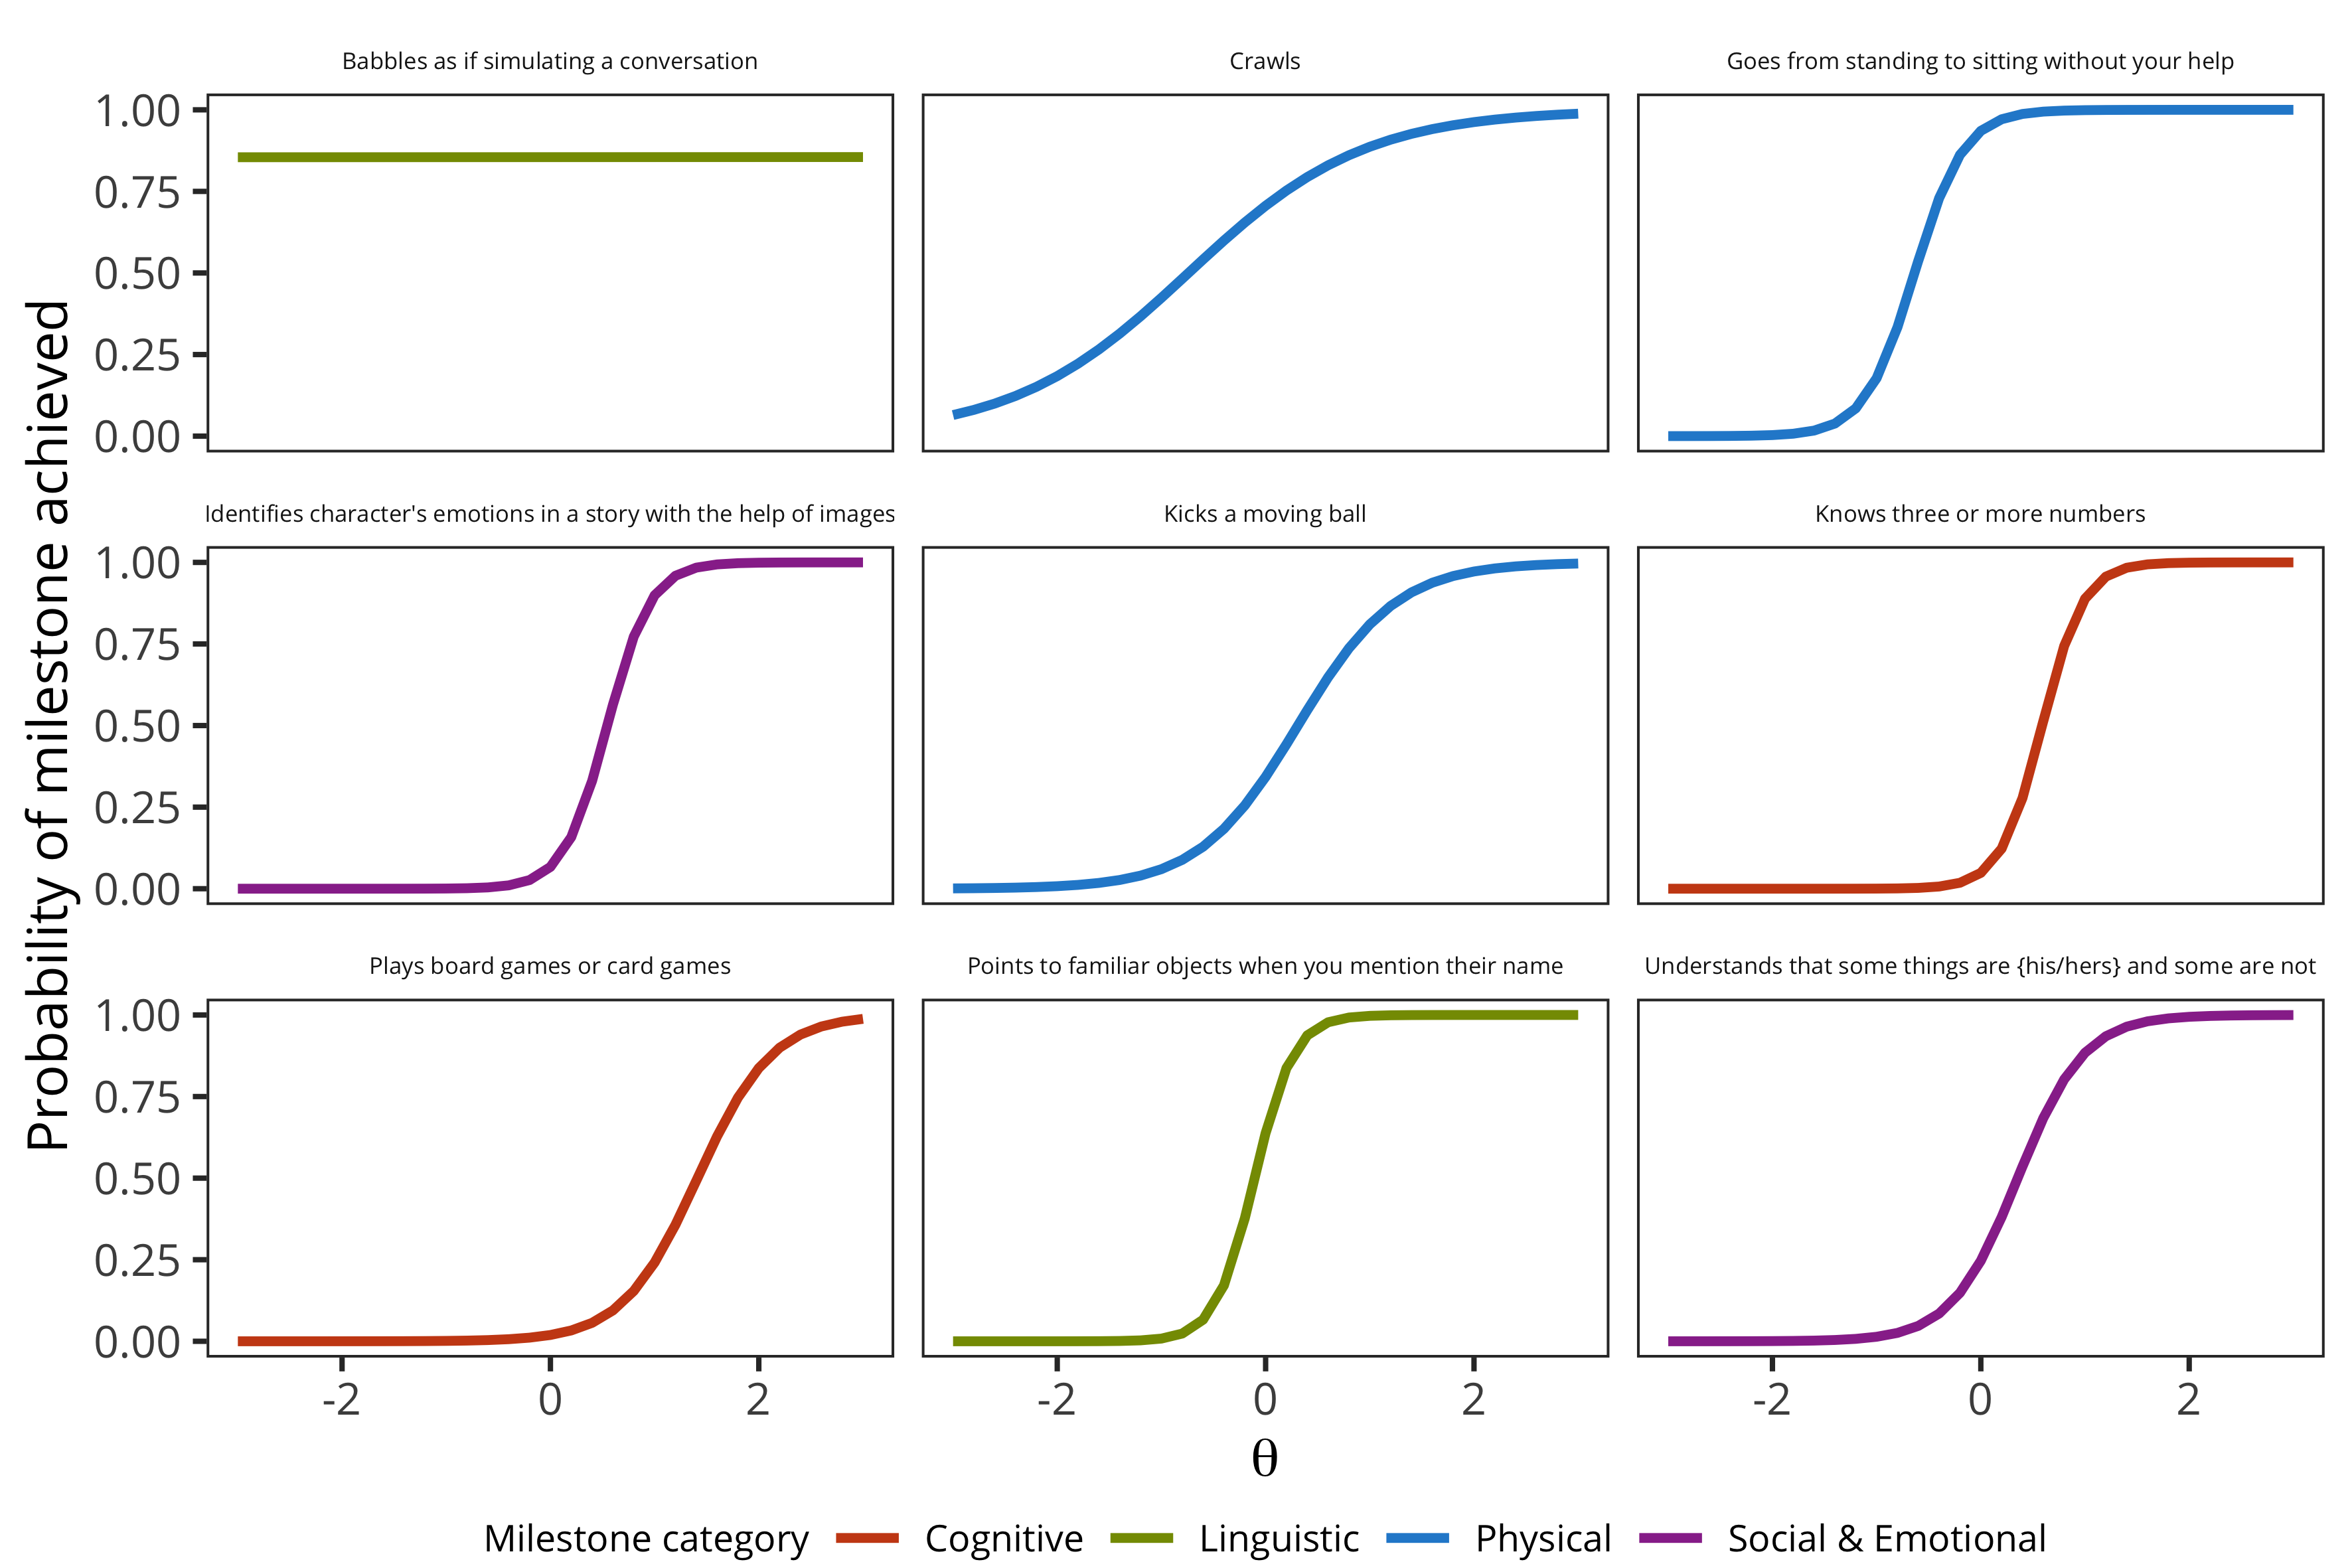
\includegraphics[width=\textwidth]{figures/08.png}
\caption{Example item characteristic curves for 9 of the 414 milestones from a 1F model fit to the survey data. Babbling is unrelated to a child's development whereas other milestones such as knowing three or more numbers are highly related to development.}
\label{fig:curves}
\end{figure}

\begin{figure}
\centering
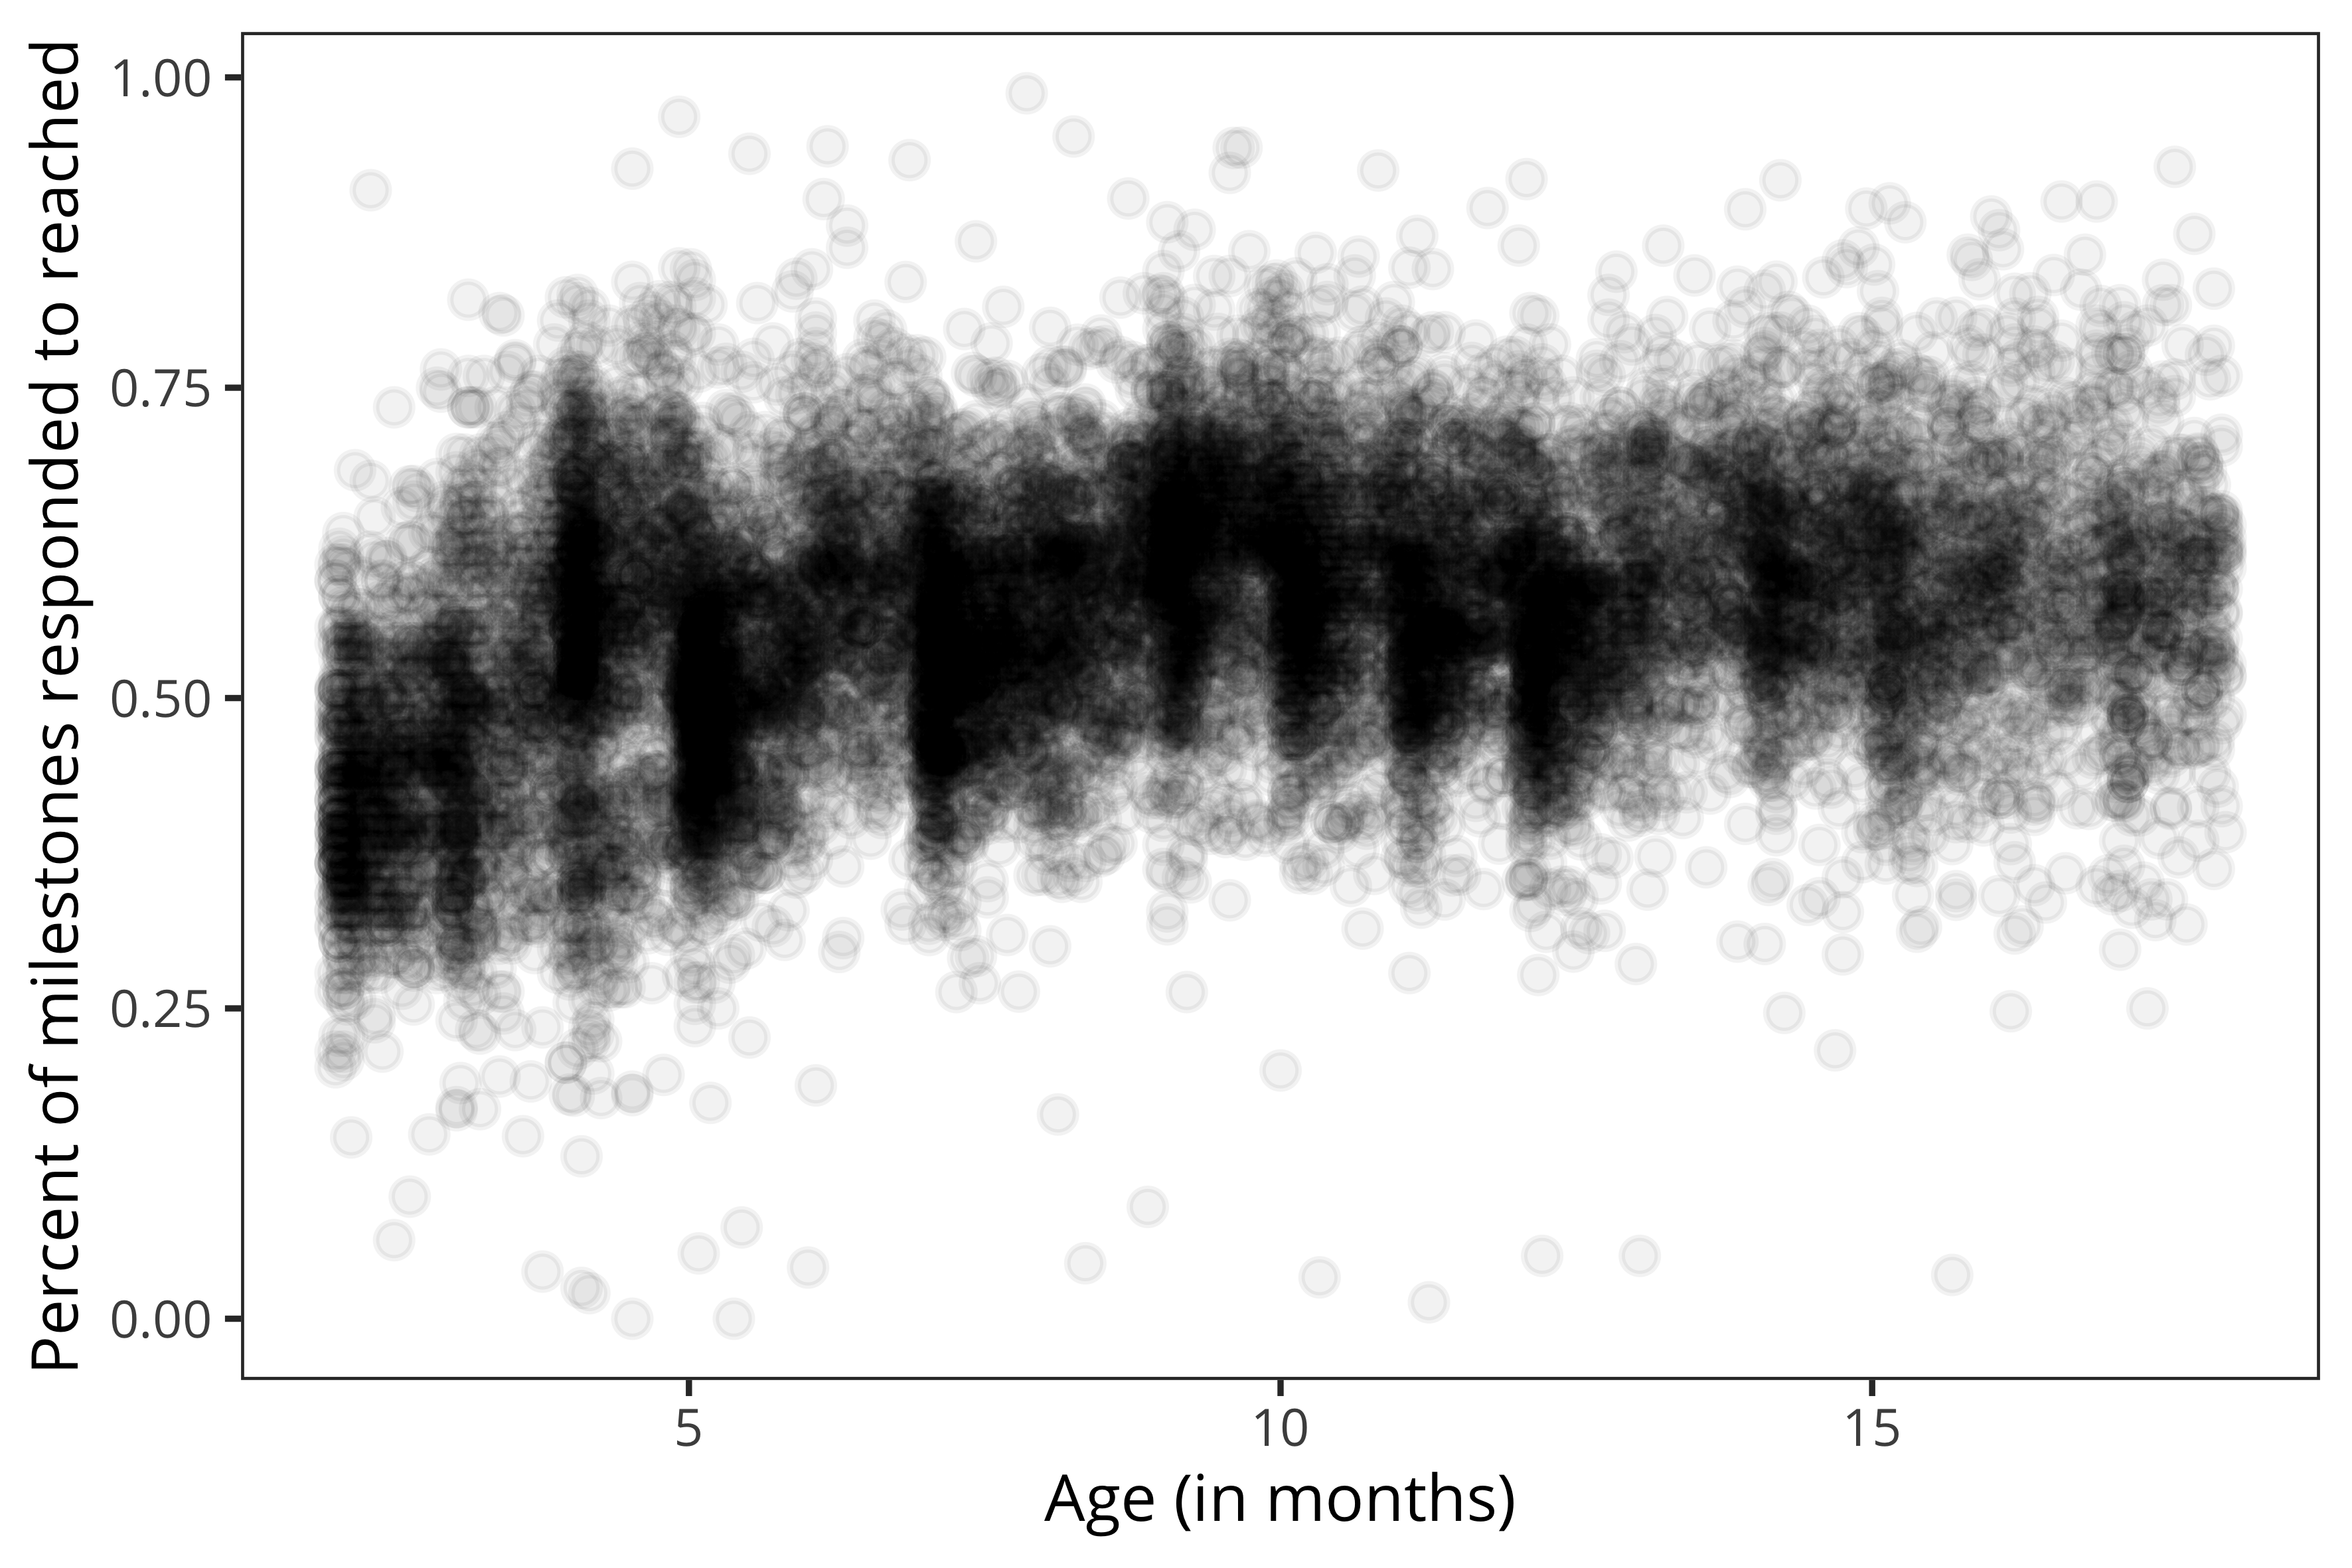
\includegraphics[width=\textwidth]{figures/rawp.png}
\caption{The raw proportion of milestones reached by age in months of the child. This proportion stays relatively constant over the age-span because as children develop the milestones that parents respond to become more advanced. As a result, ceiling effects for older children are avoided.}
\label{fig:rawp}
\end{figure}

\begin{figure}
\centering
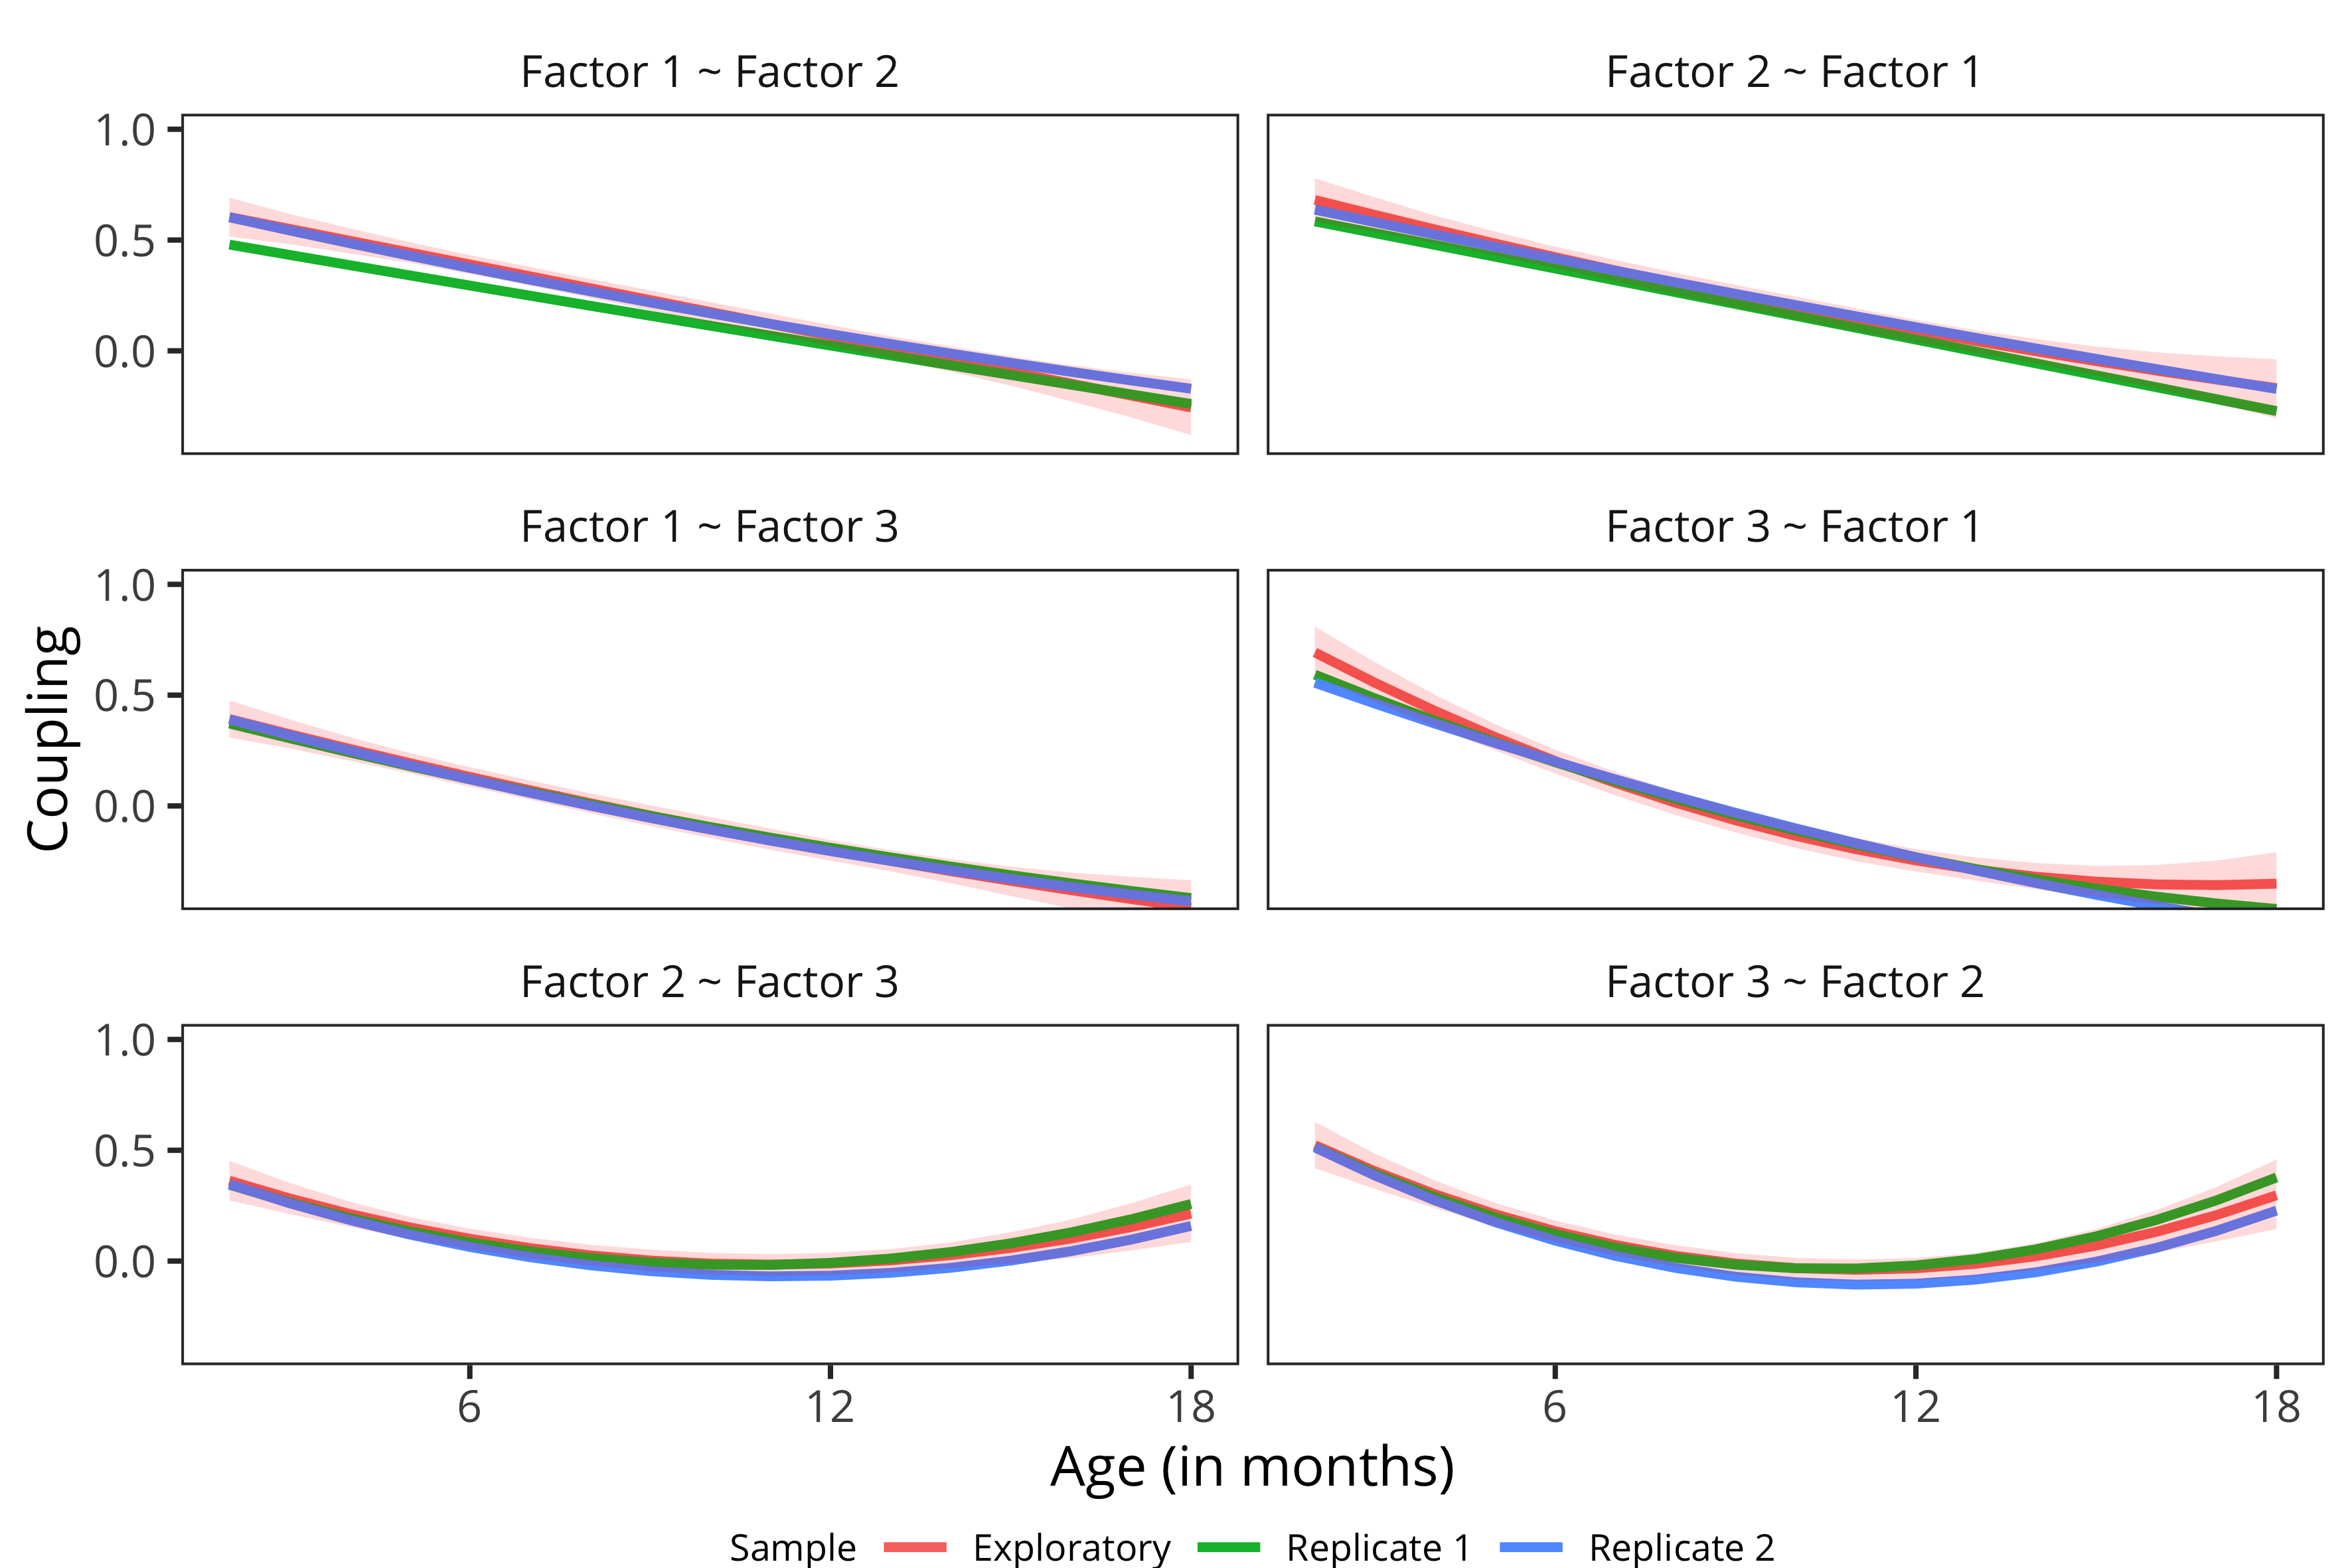
\includegraphics[width=\textwidth]{figures/04.png}
\caption{Coupling parameters from 2 to 18 months old from a 3f measurement model. Association between 1-unit deviation from the developmental pathway for one factor with deviation from the other factor’s developmental path. Top row shows the relationship between factor 1 and factor 2. Middle row shows the relationship between factor 1 and factor 3. Bottom row shows the relationship between factor 2 and factor 3. Red shading is 95\% confidence interval for exploratory sample as calculated by 1000 bootstrapped simulations. As the differentiation hypothesis suggests, we find decreasing coupling over the age span in the relationship between factor 1 and factor 2 as well as between factor 1 and factor 3.}
\label{fig:three}
\end{figure}

\begin{figure}
\centering
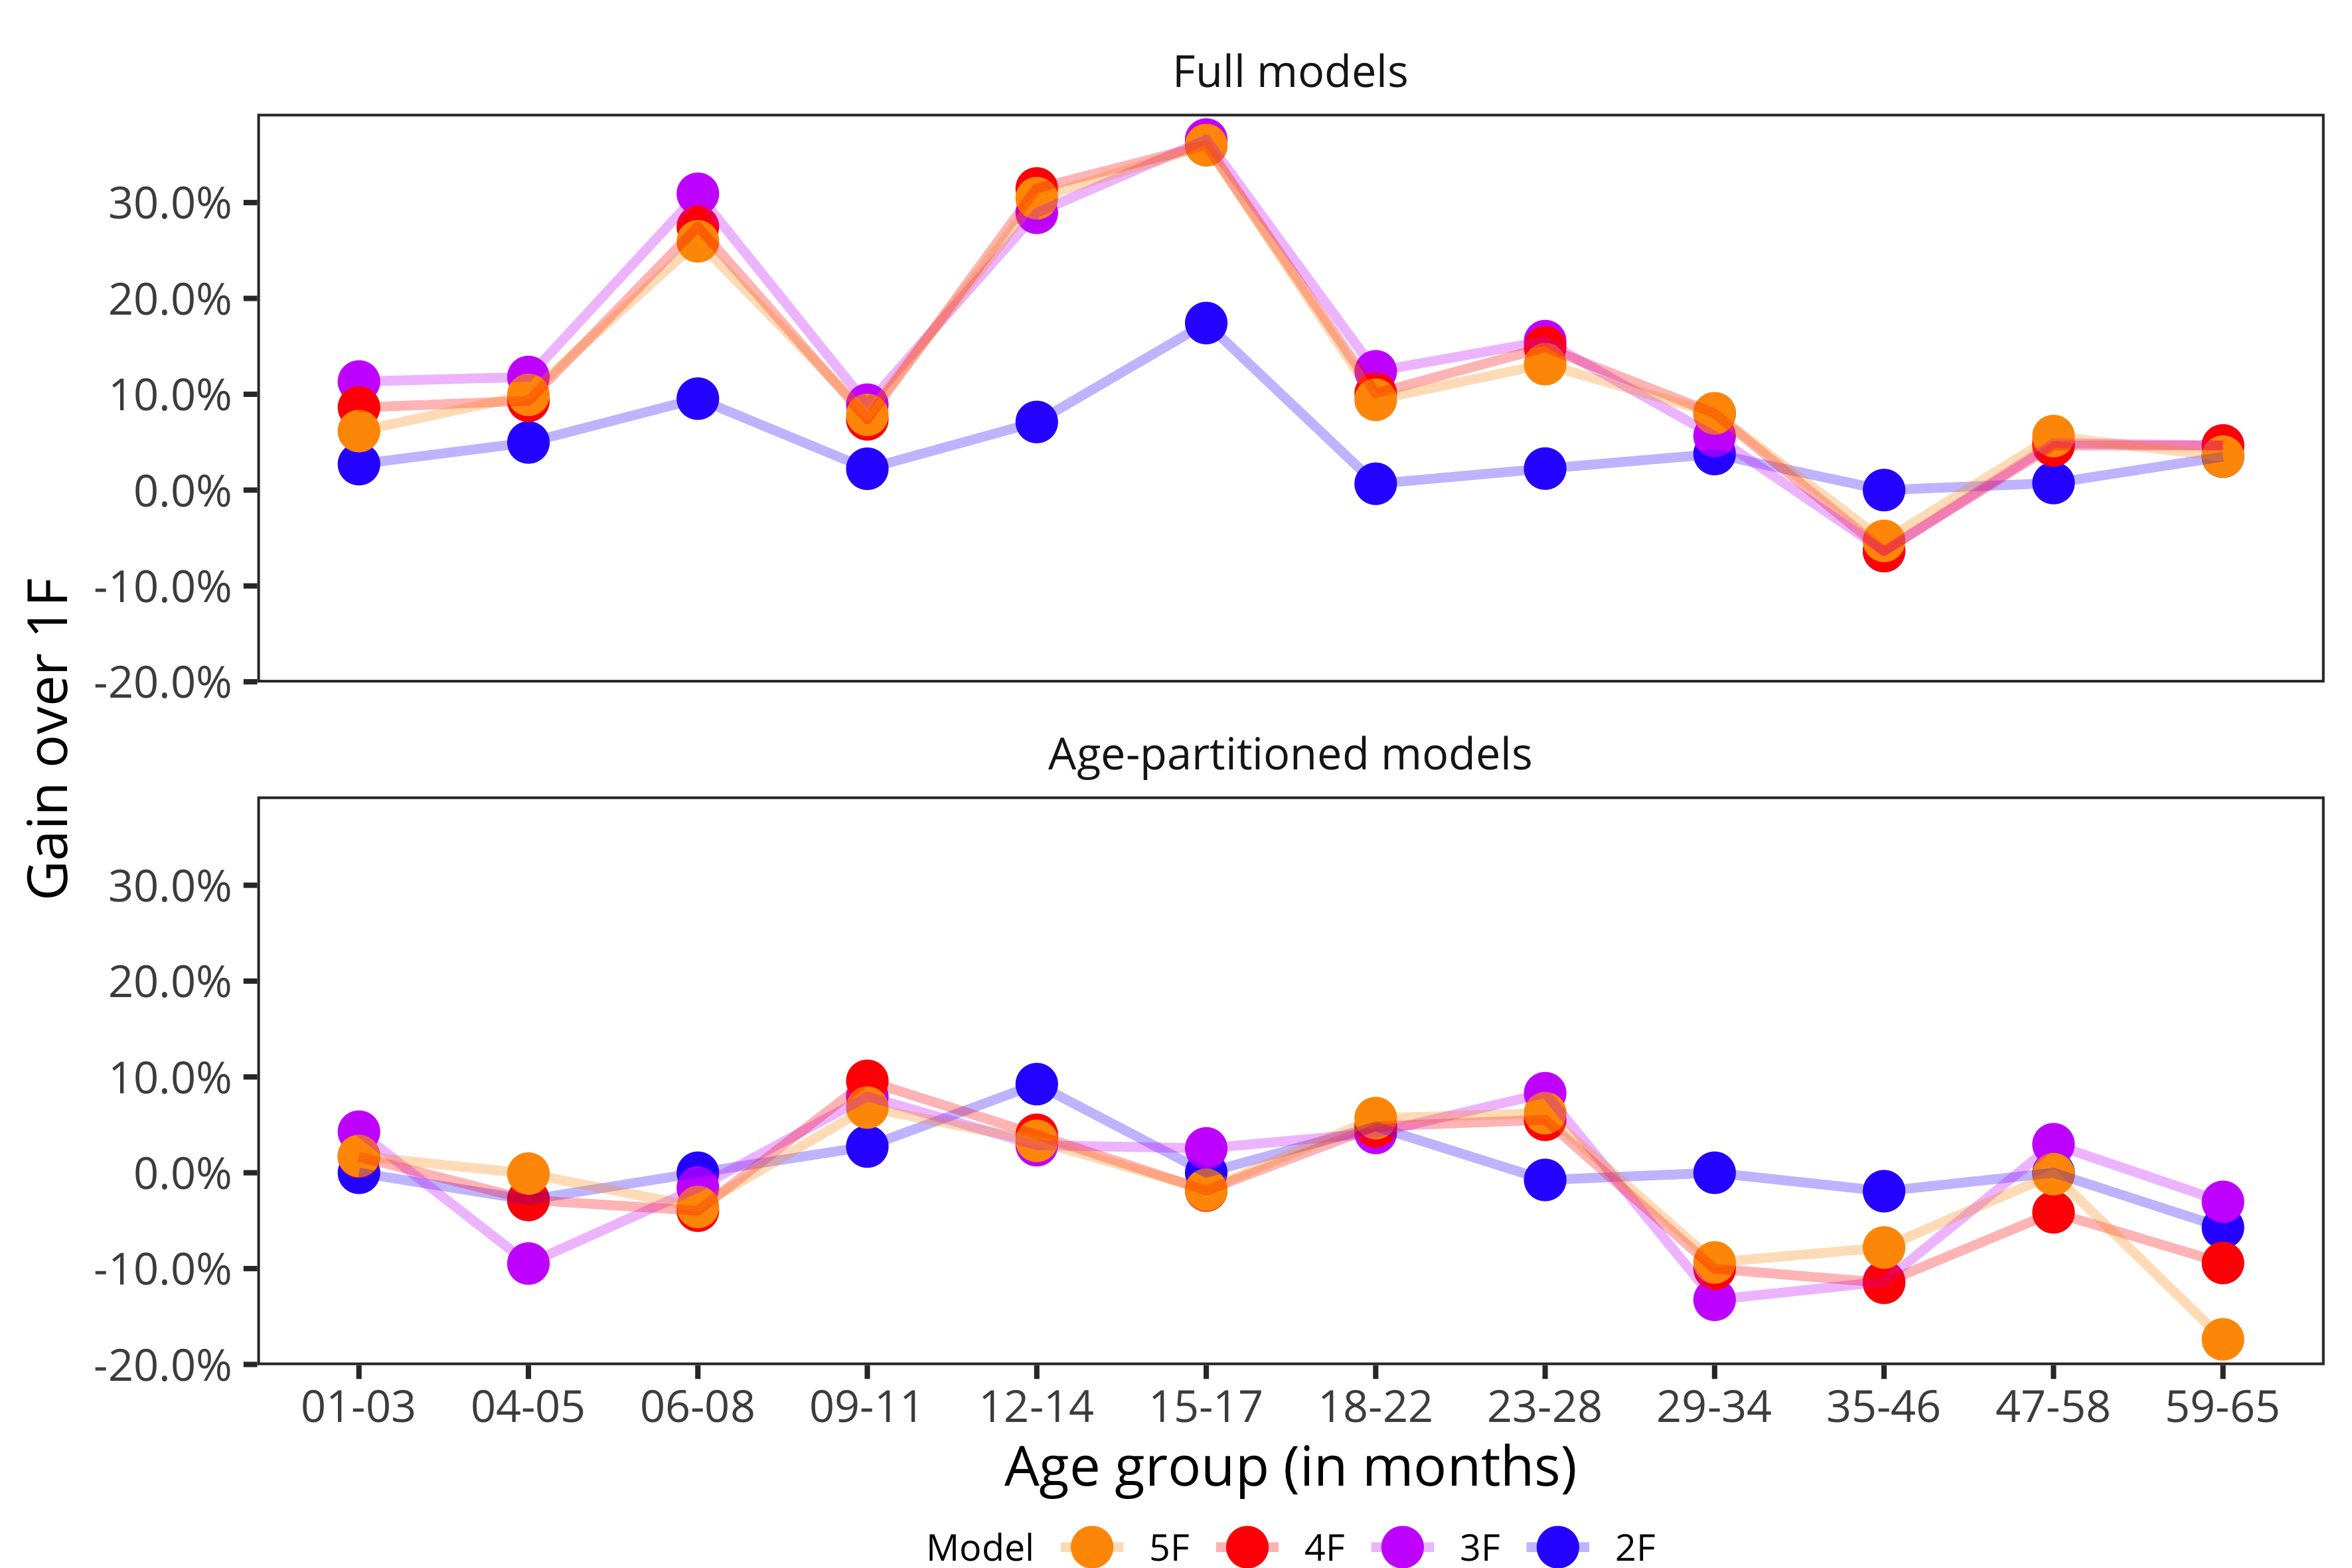
\includegraphics[width=\textwidth]{figures/06.png}
\caption{Gain of higher-dimensional models over 1F model for the SWYC data. Gain is defined as the proportion of the distance between the 1F model’s performance and 100\% that the model achieves. The top panel shows results from when each model is fit to the full dataset. The bottom panel shows results from when each model is fit separately to each age group. We did not find a consistent relationship between age (i.e., instrument version) and gain from higher dimensional models for the SWYC data.}
\label{fig:perf}
\end{figure}

\begin{figure}
\centering
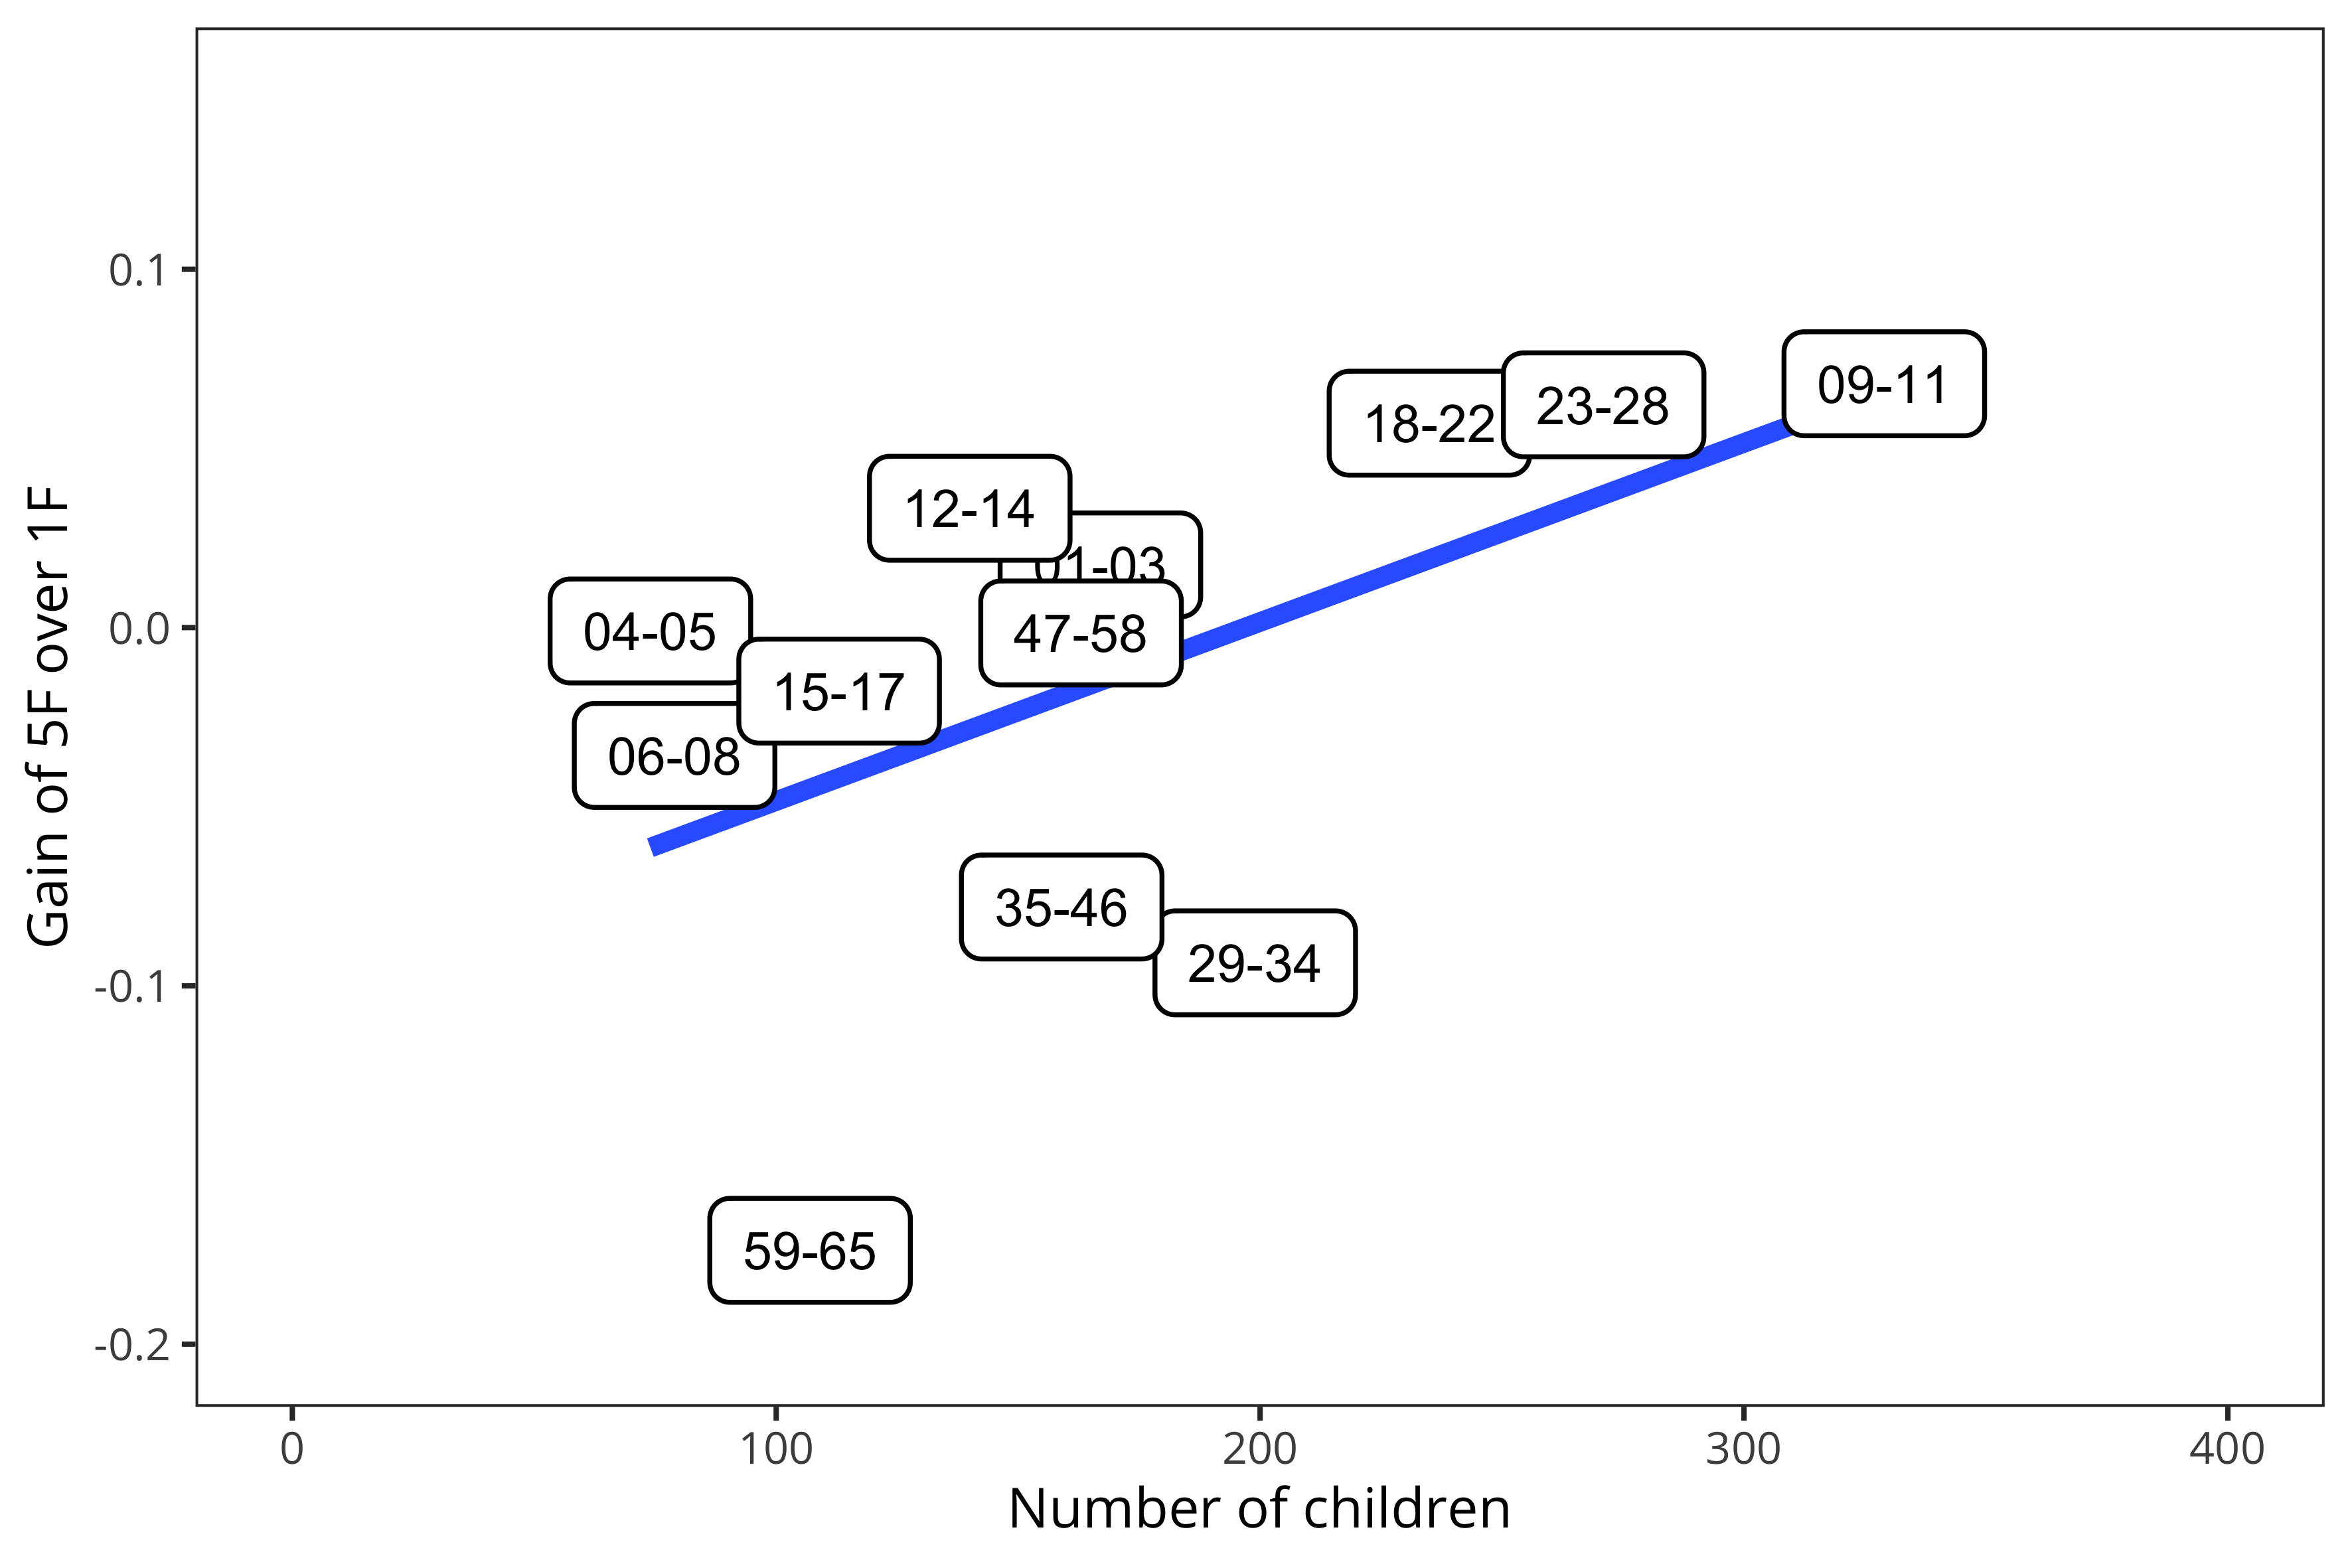
\includegraphics[width=\textwidth]{figures/07.png}
\caption{The relationship between the number of children for the SWYC version and gain between a 5F and 1F model. As expected, the 5F model performs better when fit to larger sample sizes. This confounding is one possible reason that we did not find a relationship between age group and gain over the 1F model in the previous figure.}
\label{fig:confound}
\end{figure}

%%% Add this line AFTER all your figures and tables
\FloatBarrier

All datasets are provided by Kinedu, Inc. We ask that you notify Kinedu, Inc. before using any of the datasets by emailing luis@kinedu.com. \\\\
\dataset{milestones.csv}{Kinedu's milestones. Each row corresponds to one of 422 milestones (8 milestones were not used after 2017). Columns as follows: \\\\
- milestone: A unique number that identifies the milestone \\
- area: One of the four milestone categories \\
- short: The short milestone identifier \\
- long: The full milestone description \\
- start: The targeted age (in months) that a child should be able to achieve the milestone.}

\dataset{survey.csv}{The survey data focused on in Study 1 and to develop the measurement model in Study 2. The first column is the age in months of the child. The additional 414 columns correspond to milestones. Names of these columns match to the "short" column from milestones.csv.}

\dataset{babies.csv}{Kinedu's user data as collected when a parent first creates an account. Each row is a child in the app data. Columns as follows: \\\\
- id: The child's unique identifier. Corresponds to babyid in app#.csv \\
- birthday: The date of the child's birth as reported by the parent \\
- gender: The gender of the child as reported by the parent}

\dataset{app#.csv}{Kinedu's database data as collected by parents' use of their mobile application. Due to size, this dataset is split into five files: app1.csv, app2.csv, app3.csv, app4.csv, and app5.csv. Columns as follows: \\\\
- milestone\_id: The milestone identifier. Corresponds to "milestone" from milestones.csv \\
- baby\_id: A unique identifier for the child responses regard \\
- answer: Whether the child has achieved the milestone \\
- baby\_age: The age of the child (in days) at the time of the response \\
- update\_count: The number of times the parent has updated their initial response \\
- created\_at: The date and time of the parent's inital response \\
- updated\_at: The most recent time that the parent edited their response (same as created\_at if not updated)}

\dataset{samples.csv}{The babies used for each of the three samples in the paper. Columns as follows: \\\\
- exploratory: The sample of 600 babyids that we used while developing methods \\
- replication1: The first sample of 600 babyids that methods were replicated with  \\
- replication2: The second sample of 600 babyids that methods were replicated with}


\bibliography{pnas-sample}

\end{document}
